%% Copyright 2005 G. W. Knor
%%This work may be distributed and/or modified under the
% conditions of the LaTeX Project Public License, either version 1.3
% of this license or (at your option) any later version.
% The latest version of this license is in
% http://www.latex-project.org/lppl.txt
% and version 1.3 or later is part of all distributions of LaTeX
% version 2005/12/01 or later.
%%This work has the LPPL maintenance status "maintained".
%%The Current Maintainer of this work is G. W. Knor.

\documentclass{beamer}
\usepackage{graphicx}
\usepackage{amsmath} % provides \text{<stuff>} which prints <stuff> in text mode
\usepackage{sidecap}
\usepackage{courier}
\usepackage{listings}
\usepackage{hyperref}
\usepackage[utf8]
{inputenc}
\lstset{
    breaklines=true,
    breakatwhitespace=true,
    postbreak=\raisebox{0ex}[0ex][0ex]{
        \ensuremath{
            \color{red}\hookrightarrow\space
        }
    }
}
\setcounter{tocdepth}{1}

\definecolor{keywords}{RGB}{255,0,90}
\definecolor{comments}{RGB}{0,0,113}
\definecolor{red}{RGB}{160,0,0}
\definecolor{green}{RGB}{0,150,0}

\lstset{
    language=Python,
    basicstyle=\ttfamily\footnotesize,
    keywordstyle=\color{keywords},
    commentstyle=\color{comments},
    stringstyle=\color{red},
    showstringspaces=false,
    identifierstyle=\color{green}
}


\title{HowTo re}
\author{Dariusz Śmigiel}
\date{PyCon PL 2015}
\usetheme{Warsaw}
\usecolortheme{beaver}

\begin{document}

\begin{frame}
\titlepage
\end{frame}

\section{History}
\subsection{Origins}
\begin{frame}
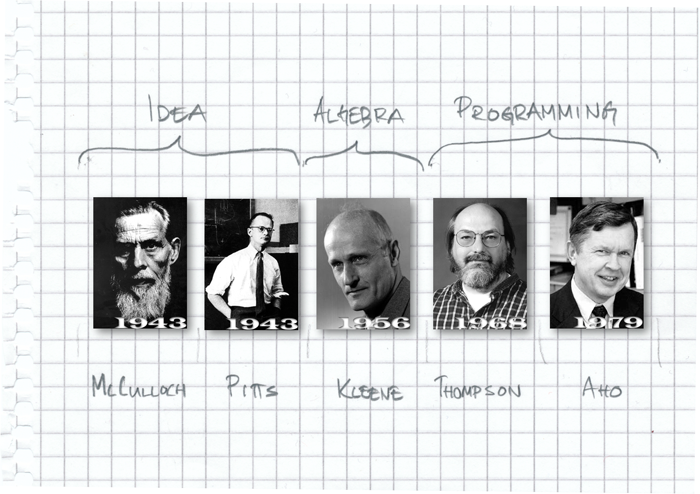
\includegraphics[width=1\textwidth]{images/history.png}
\end{frame}

\subsection{re module}
\begin{frame}
Delivering Quality since December 31, 1997 \\
\pause
Release of Python 1.5
\pause

\begin{itemize}
 \item Deprecated old module `regex`, based on Perl-style patterns.
\pause
 \item `regex` finally removed in Python 2.5.
\end{itemize}
\end{frame}

\section{Do I need it?}
\subsection{Matching / Modifying}
\begin{frame}
Answer for questions:
 \begin{itemize}
  \item "Does this string match the pattern?"
  \item "Is there a match for the pattern anywhere in this string?"
 \end{itemize}
 \pause
 \begin{itemize}
  \item Replace part of it
  \item Split into pieces
 \end{itemize}
\end{frame}

\section{Under the hood}
\subsection{Implementation / Features}
\begin{frame}[fragile]
 re is handled as string  - there is no special syntax for expressing it (advantage and disadvantage) \\
 \pause
 re patterns are compiled into bytecode \\
 \pause
 re module is a C extension module (like \verb/socket/ or \verb/zlib/) \\
 \pause
 re language is relatively small and restricted
 \pause
 \begin{itemize}
  \item not all possible string processing tasks can be done
  \item some of them can be done, but expression would be very complicated
 \end{itemize}
\end{frame}

\subsection{Regex Example}
\begin{frame}[fragile]
\begingroup
 \fontsize{6pt}{8pt}\selectfont
\begin{verbatim}
(?:(?:\r\n)?[ \t])*(?:(?:(?:[^()<>@,;:\\".\[\] \000-\031]+(?:(?:(?:\r\n)?[ \t]
)+|\Z|(?=[\["()<>@,;:\\".\[\]]))|"(?:[^\"\r\\]|\\.|(?:(?:\r\n)?[ \t]))*"(?:(?:
\r\n)?[ \t])*)(?:\.(?:(?:\r\n)?[ \t])*(?:[^()<>@,;:\\".\[\] \000-\031]+(?:(?:(
?:\r\n)?[ \t])+|\Z|(?=[\["()<>@,;:\\".\[\]]))|"(?:[^\"\r\\]|\\.|(?:(?:\r\n)?[
\t]))*"(?:(?:\r\n)?[ \t])*))*@(?:(?:\r\n)?[ \t])*(?:[^()<>@,;:\\".\[\] \000-\0
31]+(?:(?:(?:\r\n)?[ \t])+|\Z|(?=[\["()<>@,;:\\".\[\]]))|\[([^\[\]\r\\]|\\.)*\
](?:(?:\r\n)?[ \t])*)(?:\.(?:(?:\r\n)?[ \t])*(?:[^()<>@,;:\\".\[\] \000-\031]+
(?:(?:(?:\r\n)?[ \t])+|\Z|(?=[\["()<>@,;:\\".\[\]]))|\[([^\[\]\r\\]|\\.)*\](?:
(?:\r\n)?[ \t])*))*|(?:[^()<>@,;:\\".\[\] \000-\031]+(?:(?:(?:\r\n)?[ \t])+|\Z
|(?=[\["()<>@,;:\\".\[\]]))|"(?:[^\"\r\\]|\\.|(?:(?:\r\n)?[ \t]))*"(?:(?:\r\n)
?[ \t])*)*\<(?:(?:\r\n)?[ \t])*(?:@(?:[^()<>@,;:\\".\[\] \000-\031]+(?:(?:(?:\
r\n)?[ \t])+|\Z|(?=[\["()<>@,;:\\".\[\]]))|\[([^\[\]\r\\]|\\.)*\](?:(?:\r\n)?[
 \t])*)(?:\.(?:(?:\r\n)?[ \t])*(?:[^()<>@,;:\\".\[\] \000-\031]+(?:(?:(?:\r\n)
?[ \t])+|\Z|(?=[\["()<>@,;:\\".\[\]]))|\[([^\[\]\r\\]|\\.)*\](?:(?:\r\n)?[ \t]
)*))*(?:,@(?:(?:\r\n)?[ \t])*(?:[^()<>@,;:\\".\[\] \000-\031]+(?:(?:(?:\r\n)?[
 \t])+|\Z|(?=[\["()<>@,;:\\".\[\]]))|\[([^\[\]\r\\]|\\.)*\](?:(?:\r\n)?[ \t])*
)(?:\.(?:(?:\r\n)?[ \t])*(?:[^()<>@,;:\\".\[\] \000-\031]+(?:(?:(?:\r\n)?[ \t]
)+|\Z|(?=[\["()<>@,;:\\".\[\]]))|\[([^\[\]\r\\]|\\.)*\](?:(?:\r\n)?[ \t])*))*)
*:(?:(?:\r\n)?[ \t])*)?(?:[^()<>@,;:\\".\[\] \000-\031]+(?:(?:(?:\r\n)?[ \t])+
|\Z|(?=[\["()<>@,;:\\".\[\]]))|"(?:[^\"\r\\]|\\.|(?:(?:\r\n)?[ \t]))*"(?:(?:\r
\n)?[ \t])*)(?:\.(?:(?:\r\n)?[ \t])*(?:[^()<>@,;:\\".\[\] \000-\031]+(?:(?:(?:
\end{verbatim}
 \endgroup
\end{frame}

\begin{frame}[fragile]
\begingroup
 \fontsize{6pt}{8pt}\selectfont
\begin{verbatim}
\r\n)?[ \t])+|\Z|(?=[\["()<>@,;:\\".\[\]]))|"(?:[^\"\r\\]|\\.|(?:(?:\r\n)?[ \t
]))*"(?:(?:\r\n)?[ \t])*))*@(?:(?:\r\n)?[ \t])*(?:[^()<>@,;:\\".\[\] \000-\031
]+(?:(?:(?:\r\n)?[ \t])+|\Z|(?=[\["()<>@,;:\\".\[\]]))|\[([^\[\]\r\\]|\\.)*\](
?:(?:\r\n)?[ \t])*)(?:\.(?:(?:\r\n)?[ \t])*(?:[^()<>@,;:\\".\[\] \000-\031]+(?
:(?:(?:\r\n)?[ \t])+|\Z|(?=[\["()<>@,;:\\".\[\]]))|\[([^\[\]\r\\]|\\.)*\](?:(?
:\r\n)?[ \t])*))*\>(?:(?:\r\n)?[ \t])*)|(?:[^()<>@,;:\\".\[\] \000-\031]+(?:(?
:(?:\r\n)?[ \t])+|\Z|(?=[\["()<>@,;:\\".\[\]]))|"(?:[^\"\r\\]|\\.|(?:(?:\r\n)?
[ \t]))*"(?:(?:\r\n)?[ \t])*)*:(?:(?:\r\n)?[ \t])*(?:(?:(?:[^()<>@,;:\\".\[\]
\000-\031]+(?:(?:(?:\r\n)?[ \t])+|\Z|(?=[\["()<>@,;:\\".\[\]]))|"(?:[^\"\r\\]|
\\.|(?:(?:\r\n)?[ \t]))*"(?:(?:\r\n)?[ \t])*)(?:\.(?:(?:\r\n)?[ \t])*(?:[^()<>
@,;:\\".\[\] \000-\031]+(?:(?:(?:\r\n)?[ \t])+|\Z|(?=[\["()<>@,;:\\".\[\]]))|"
(?:[^\"\r\\]|\\.|(?:(?:\r\n)?[ \t]))*"(?:(?:\r\n)?[ \t])*))*@(?:(?:\r\n)?[ \t]
)*(?:[^()<>@,;:\\".\[\] \000-\031]+(?:(?:(?:\r\n)?[ \t])+|\Z|(?=[\["()<>@,;:\\
".\[\]]))|\[([^\[\]\r\\]|\\.)*\](?:(?:\r\n)?[ \t])*)(?:\.(?:(?:\r\n)?[ \t])*(?
:[^()<>@,;:\\".\[\] \000-\031]+(?:(?:(?:\r\n)?[ \t])+|\Z|(?=[\["()<>@,;:\\".\[
\]]))|\[([^\[\]\r\\]|\\.)*\](?:(?:\r\n)?[ \t])*))*|(?:[^()<>@,;:\\".\[\] \000-
\031]+(?:(?:(?:\r\n)?[ \t])+|\Z|(?=[\["()<>@,;:\\".\[\]]))|"(?:[^\"\r\\]|\\.|(
?:(?:\r\n)?[ \t]))*"(?:(?:\r\n)?[ \t])*)*\<(?:(?:\r\n)?[ \t])*(?:@(?:[^()<>@,;
:\\".\[\] \000-\031]+(?:(?:(?:\r\n)?[ \t])+|\Z|(?=[\["()<>@,;:\\".\[\]]))|\[([
^\[\]\r\\]|\\.)*\](?:(?:\r\n)?[ \t])*)(?:\.(?:(?:\r\n)?[ \t])*(?:[^()<>@,;:\\"
.\[\] \000-\031]+(?:(?:(?:\r\n)?[ \t])+|\Z|(?=[\["()<>@,;:\\".\[\]]))|\[([^\[\
\end{verbatim}
 \endgroup
\end{frame}

\begin{frame}[fragile]
\begingroup
 \fontsize{6pt}{8pt}\selectfont
\begin{verbatim}
]\r\\]|\\.)*\](?:(?:\r\n)?[ \t])*))*(?:,@(?:(?:\r\n)?[ \t])*(?:[^()<>@,;:\\".\
[\] \000-\031]+(?:(?:(?:\r\n)?[ \t])+|\Z|(?=[\["()<>@,;:\\".\[\]]))|\[([^\[\]\
r\\]|\\.)*\](?:(?:\r\n)?[ \t])*)(?:\.(?:(?:\r\n)?[ \t])*(?:[^()<>@,;:\\".\[\]
\000-\031]+(?:(?:(?:\r\n)?[ \t])+|\Z|(?=[\["()<>@,;:\\".\[\]]))|\[([^\[\]\r\\]
|\\.)*\](?:(?:\r\n)?[ \t])*))*)*:(?:(?:\r\n)?[ \t])*)?(?:[^()<>@,;:\\".\[\] \0
00-\031]+(?:(?:(?:\r\n)?[ \t])+|\Z|(?=[\["()<>@,;:\\".\[\]]))|"(?:[^\"\r\\]|\\
.|(?:(?:\r\n)?[ \t]))*"(?:(?:\r\n)?[ \t])*)(?:\.(?:(?:\r\n)?[ \t])*(?:[^()<>@,
;:\\".\[\] \000-\031]+(?:(?:(?:\r\n)?[ \t])+|\Z|(?=[\["()<>@,;:\\".\[\]]))|"(?
:[^\"\r\\]|\\.|(?:(?:\r\n)?[ \t]))*"(?:(?:\r\n)?[ \t])*))*@(?:(?:\r\n)?[ \t])*
(?:[^()<>@,;:\\".\[\] \000-\031]+(?:(?:(?:\r\n)?[ \t])+|\Z|(?=[\["()<>@,;:\\".
\[\]]))|\[([^\[\]\r\\]|\\.)*\](?:(?:\r\n)?[ \t])*)(?:\.(?:(?:\r\n)?[ \t])*(?:[
^()<>@,;:\\".\[\] \000-\031]+(?:(?:(?:\r\n)?[ \t])+|\Z|(?=[\["()<>@,;:\\".\[\]
]))|\[([^\[\]\r\\]|\\.)*\](?:(?:\r\n)?[ \t])*))*\>(?:(?:\r\n)?[ \t])*)(?:,\s*(
?:(?:[^()<>@,;:\\".\[\] \000-\031]+(?:(?:(?:\r\n)?[ \t])+|\Z|(?=[\["()<>@,;:\\
".\[\]]))|"(?:[^\"\r\\]|\\.|(?:(?:\r\n)?[ \t]))*"(?:(?:\r\n)?[ \t])*)(?:\.(?:(
?:\r\n)?[ \t])*(?:[^()<>@,;:\\".\[\] \000-\031]+(?:(?:(?:\r\n)?[ \t])+|\Z|(?=[
\["()<>@,;:\\".\[\]]))|"(?:[^\"\r\\]|\\.|(?:(?:\r\n)?[ \t]))*"(?:(?:\r\n)?[ \t
])*))*@(?:(?:\r\n)?[ \t])*(?:[^()<>@,;:\\".\[\] \000-\031]+(?:(?:(?:\r\n)?[ \t
])+|\Z|(?=[\["()<>@,;:\\".\[\]]))|\[([^\[\]\r\\]|\\.)*\](?:(?:\r\n)?[ \t])*)(?
:\.(?:(?:\r\n)?[ \t])*(?:[^()<>@,;:\\".\[\] \000-\031]+(?:(?:(?:\r\n)?[ \t])+|
\Z|(?=[\["()<>@,;:\\".\[\]]))|\[([^\[\]\r\\]|\\.)*\](?:(?:\r\n)?[ \t])*))*|(?:
\end{verbatim}
 \endgroup
\end{frame}

\begin{frame}[fragile]
\begingroup
 \fontsize{6pt}{8pt}\selectfont
\begin{verbatim}
[^()<>@,;:\\".\[\] \000-\031]+(?:(?:(?:\r\n)?[ \t])+|\Z|(?=[\["()<>@,;:\\".\[\
]]))|"(?:[^\"\r\\]|\\.|(?:(?:\r\n)?[ \t]))*"(?:(?:\r\n)?[ \t])*)*\<(?:(?:\r\n)
?[ \t])*(?:@(?:[^()<>@,;:\\".\[\] \000-\031]+(?:(?:(?:\r\n)?[ \t])+|\Z|(?=[\["
()<>@,;:\\".\[\]]))|\[([^\[\]\r\\]|\\.)*\](?:(?:\r\n)?[ \t])*)(?:\.(?:(?:\r\n)
?[ \t])*(?:[^()<>@,;:\\".\[\] \000-\031]+(?:(?:(?:\r\n)?[ \t])+|\Z|(?=[\["()<>
@,;:\\".\[\]]))|\[([^\[\]\r\\]|\\.)*\](?:(?:\r\n)?[ \t])*))*(?:,@(?:(?:\r\n)?[
 \t])*(?:[^()<>@,;:\\".\[\] \000-\031]+(?:(?:(?:\r\n)?[ \t])+|\Z|(?=[\["()<>@,
;:\\".\[\]]))|\[([^\[\]\r\\]|\\.)*\](?:(?:\r\n)?[ \t])*)(?:\.(?:(?:\r\n)?[ \t]
)*(?:[^()<>@,;:\\".\[\] \000-\031]+(?:(?:(?:\r\n)?[ \t])+|\Z|(?=[\["()<>@,;:\\
".\[\]]))|\[([^\[\]\r\\]|\\.)*\](?:(?:\r\n)?[ \t])*))*)*:(?:(?:\r\n)?[ \t])*)?
(?:[^()<>@,;:\\".\[\] \000-\031]+(?:(?:(?:\r\n)?[ \t])+|\Z|(?=[\["()<>@,;:\\".
\[\]]))|"(?:[^\"\r\\]|\\.|(?:(?:\r\n)?[ \t]))*"(?:(?:\r\n)?[ \t])*)(?:\.(?:(?:
\r\n)?[ \t])*(?:[^()<>@,;:\\".\[\] \000-\031]+(?:(?:(?:\r\n)?[ \t])+|\Z|(?=[\[
"()<>@,;:\\".\[\]]))|"(?:[^\"\r\\]|\\.|(?:(?:\r\n)?[ \t]))*"(?:(?:\r\n)?[ \t])
*))*@(?:(?:\r\n)?[ \t])*(?:[^()<>@,;:\\".\[\] \000-\031]+(?:(?:(?:\r\n)?[ \t])
+|\Z|(?=[\["()<>@,;:\\".\[\]]))|\[([^\[\]\r\\]|\\.)*\](?:(?:\r\n)?[ \t])*)(?:\
.(?:(?:\r\n)?[ \t])*(?:[^()<>@,;:\\".\[\] \000-\031]+(?:(?:(?:\r\n)?[ \t])+|\Z
|(?=[\["()<>@,;:\\".\[\]]))|\[([^\[\]\r\\]|\\.)*\](?:(?:\r\n)?[ \t])*))*\>(?:(
?:\r\n)?[ \t])*))*)?;\s*)
\end{verbatim}
 \endgroup
Perl regex to validate email addresses according to the RFC 822
\url{http://ex-parrot.com/~pdw/Mail-RFC822-Address}
\end{frame}

\section{Simple patterns}
\subsection{Metacharacters}
\begin{frame}[fragile]
\begin{verbatim}
. ^ $ * + ? { } [ ] \ | ( )
\end{verbatim}
\end{frame}

\subsubsection{Class}
\begin{frame}[fragile]
\begin{verbatim}
[ ]
\end{verbatim}
Specifying a character class, which is set of characters that you wish to match
 \begin{itemize}
  \item can be listed individually \verb/[abc]/
  \item can be given as range of characters, separated by '-' \verb/[a-c]/
 \end{itemize}
\pause
Metacharacters are not active inside class \\
\verb/[akm$]/ will match any of: "a", "k", "m", "\$"
\end{frame}

\subsubsection{Complementing set}
\begin{frame}[fragile]
\begin{verbatim}
^
\end{verbatim}
Including \verb/^/ as first character of the class \verb/[^5]/ will match any except '5'
\end{frame}

\subsubsection{Dot - '.'}
\begin{frame}[fragile]
\begin{verbatim}
.
\end{verbatim}
By default, matches anything except newline character. \\
\pause
There is alternate mode (re.DOTALL) where it matches everything. Used when it's needed to match "any character"
\end{frame}

\subsection{Repeating Things}
\subsubsection{*, +, ?}
\begin{frame}[fragile]
\begin{verbatim}
*
\end{verbatim}
Doesn't match a character. Specifies that previous character can be matched zero or more times.
\begin{verbatim}
(ca*t) --> "ct", "cat", "caaat"
\end{verbatim}
\pause
\begin{verbatim}
+
\end{verbatim}
Similar to \verb/*/, but requires at least one occurence of character
\begin{verbatim}
(ca+t) --> "cat", "caaat", not "ct"
\end{verbatim}
\pause
\begin{verbatim}
?
\end{verbatim}
Matches either once or zero times
\begin{verbatim}
(ca?t) --> "ct", "cat", not "caaat"
\end{verbatim}
\pause
\begin{verbatim}
(home-?brew) --> "homebrew", "home-brew"
\end{verbatim}
\end{frame}

\subsubsection{"{m,n}"}
\begin{frame}[fragile]
\begin{verbatim}
{m,n}
\end{verbatim}
\verb/m/ and \verb/n/ are decimal numbers. There must be at least m repetitions, and at most n.
\begin{verbatim}
a/{1,3}b --> a/b, a//b, a///b
\end{verbatim}
\pause
\verb/m/ and \verb/n/ can be ommited. When m ommited, there is zero, when n ommited, upper bound infinity (more precisely, 2 billions)
\end{frame}

\subsection{Equivalents}
\begin{frame}[fragile]
\begin{verbatim}
{0,} == "*"
{1,} == "+"
{,1} == {0,1} == "?"
\end{verbatim}
\end{frame}

\subsection{Greedy}
\begin{frame}[fragile]
\verb/*/, \verb/+/ and \verb/?/ are greedy. Will try to repeat it as many times as possible (re engine can match only 2 billion characters (2GB) -- C \verb/int/ limitation). \\
\pause
\verb/a[bcd]*b/ - matches \verb/a/, zero or more letters from \verb/bcd/, and ends with \verb/b/ \\
\pause
\verb/abcbd/
\pause
\begin{itemize}
\item matches \verb/a/
\pause
\item matches \verb/abcbd/ to the end of the string
\pause
\item fails, because current position is the end of the string, so cannot match \verb/b/
\pause
\item matches \verb/abcb/ - one less character
\pause
\item fails, because current position is \verb/d/, so cannot match \verb/b/
\pause
\item matches \verb/abc/, so \verb/[bcd]*/ matches only \verb/bc/
\pause
\item \verb/abcb/, tries last character \verb/b/, and it's on current position
\pause
\item success
\end{itemize}
\end{frame}

\subsection{Non-greedy}
\begin{frame}[fragile]
\verb/*?, +?, ??, {m,n}?/ are non-greedy. Will try to match as few characters as possible.
\pause

\begin{lstlisting}
In [1]: import re

In [2]: greedy_re = re.compile("<.*>")

In [3]: text = "<html><head><title>Title</title></head></html>"

In [4]: greedy_re.findall(text)
Out[4]: ['<html><head><title>Title</title></head></html>']
\end{lstlisting}
\pause

\begin{lstlisting}
In [5]: non_greedy_re = re.compile("<.*?>")

In [6]: non_greedy_re.findall(text)
Out[6]: ['<html>', '<head>', '<title>', '</title>', '</head>', '</html>']
\end{lstlisting}

\end{frame}

\subsection{Backslash - escape metacharacters}
\begin{frame}[fragile]
\begin{verbatim}
\
\end{verbatim}
For matching \verb/[/ or \verb/\/ you can use \verb/\[/ or \verb/\\/ \\
\pause
Some of special sequences beginning with \verb/\/ express predefined sets of characters: set of digits, letters, everything but whitespace
\end{frame}

\begin{frame}[fragile]
\begin{itemize}
\item \verb/\d/ - any decimal digit, equivalent of \verb/[0-9]/
\item \verb/\D/ - everything but decimal digit, equivalent of \verb/[^0-9]/
\pause
\item \verb/\w/ - any alphanumeric: \verb/[a-zA-Z0-9_]/
\item \verb/\W/ - any non-alpahnumeric: \verb/[^a-zA-Z0-9_]/
\pause
\item \verb/\s/ - any whitespace character: \verb/[ \t\n\r\f\v]/ \\ (space, tab (ASCII 0x09), newline (0x0A), return (0x0D), form feed - page break(0x0C), vertical tab (0x0B))
\item \verb/\S/ - any non-whitespace character: \verb/[^ \t\n\r\f\v]/
\pause \\
NOTE! Remember that Windows text files use \verb/\r\n/ to terminate lines, while UNIX text files use \verb/\n/.
\end{itemize}
\end{frame}

\subsection{"Backslash Plague" problem}
\begin{frame}[fragile]
\begin{itemize}
\item re is handled as string
\item one of \verb/re/ metacharacters is \verb/\/
\item backslash for escaping in \verb/re/ conflicts with the same purpose in Python
\end{itemize}
\end{frame}

\begin{frame}[fragile]
\begin{tabular}{ | l | p{7cm} |}
\hline
Characters & Stage \\ \hline
\verb/\section/ & Text string to be matched \\
\verb/\\section/ & Escaped backslash for \verb/re.compile()/ \\
\verb/"\\\\section"/ & Escaped backslashes for a string literal \\
\hline
\end{tabular}
\pause
re string needs to be written as \verb/"\\\\"/ because regular expression must be \verb/\\/ and each must be escaped \verb/\\/ inside a regular Python string literal.
\pause
Solution - raw string
\begin{tabular}{ | l | p{7cm} |}
\hline
Regular string & Raw string \\ \hline
\verb/"ab*"/ & \verb/r"ab*"/ \\
\verb/"\\\\section"/ & \verb/r"\\section"/ \\
\verb/"\\w+\\s+"/ & \verb/r"\w+\s+"/ \\
\hline
\end{tabular}
\end{frame}

\section{Regular Expressions}
\subsection{Compilation}
\begin{frame}[fragile]
    \verb|dasm@hell:~$ python3|
    \begin{lstlisting}
    >>> import re
    >>> regex = re.compile('[a-zA-z0-9]+')
    >>> regex
    re.compile('[a-zA-z0-9]+')
    >>> regex.findall('Search test')
    ['Search', 'test']
    >>>
    \end{lstlisting}
\end{frame}

\begin{frame}[fragile]
    \verb|dasm@hell:~$ python3|
    \begin{lstlisting}
    >>> import re
    >>> regex = re.compile('[a-zA-z0-9]+')
    >>> regex
    re.compile('[a-zA-z0-9]+')
    >>> re.findall(regex, 'Search test 03')
    ['Search', 'test', '03']
    >>>
    \end{lstlisting}
\end{frame}

\begin{frame}[fragile]
    \verb|dasm@hell:~$ python3|
    \begin{lstlisting}
    >>> import re
    >>> re.findall('[a-zA-Z0-9]+', 'Search test 02')
    ['Search', 'test']
    >>>
    \end{lstlisting}
\end{frame}

\subsection{Compilation Flags}
\subsubsection{re.DEBUG}
\begin{frame}[fragile]
\verb/re.DEBUG/
\begin{lstlisting}
>>> import re
>>> regex = re.compile('[a-z]', re.DEBUG)
in
  range (97, 122)
>>>
\end{lstlisting}
\end{frame}

\subsubsection{re.ASCII}
\begin{frame}[fragile]
\verb/re.ASCII/ \\
\verb/\xa0/ - non-breaking space
\begin{lstlisting}
>>> import re
>>> regex = re.compile("\s+")
>>> regex.findall("\xa0 ha")
['\xa0 ']
>>> regex = re.compile("\s+", re.ASCII)
>>> regex.findall("\xa0 ha")
[' ']
>>>
\end{lstlisting}
\end{frame}

\subsection{Performing Matches}
\begin{frame}[fragile]
\end{frame}

\section{Bibliography}
\begin{frame}
\begingroup
 \fontsize{6pt}{8pt}\selectfont
\begin{itemize}
\item Regular Expression HOWTO: \url{https://docs.python.org/2/howto/regex.html}
\item Python Docs: Library re: \url{https://docs.python.org/2/library/re.html}
\item Google for Education. Python Regular Expressions: \url{https://developers.google.com/edu/python/regular-expressions?hl=en}
\item Non-printable Characters: \url{http://www.regular-expressions.info/nonprint.html}
\item Core Python Applications programming: Regular expressions: \url{http://www.informit.com/articles/article.aspx?p=1707750&seqNum=2}
\item Brief history by Staffan Noteberg: \url{http://blog.staffannoteberg.com/}
\end{itemize}
\endgroup
\end{frame}
\end{document}
